\section{Experiments and Evaluation}
\label{sec:experiments}

In this section, we evaluate our method on the TU-Berlin sketch benchmark, which is the largest human sketch dataset to data. 
%
It contains in total 20000 sketches of 250 categories. Each category has 80 instances. 
%
We do a group of experiments to compare our method with other methods in both recognition accuracy and model size (number of trainable parameters). 
%
We performed three-fold cross validation within the dataset using 
the same strategy with previous methods~\cite{Yu2015SketchaNetTB, Dupont2016DeepSketch2D}.
%Like previous works, we use 3-fold cross-validation within the dataset. 
Dataset augmentation is also performed to ease the over-fitting problem, same as~\cite{Yu2015SketchaNetTB}.
\\


\noindent \textbf{Training strategy.} 
%
Our SketchPointNet, \xjmd{which is composed of all fully-connected layers for pattern extraction,} can be trained end-to-end by back-propagation and SGD, with the softmax classification loss.
%
However, the entire network is easily converged to a local optima and suffers from overfitting. 
Moreover, the third pointnet PN-3 plays different roles from PN-1 and PN-2. It captures more global pattern for classification. 
%
\xjmd{For the multilayer perceptrons in the entire networks, we use paramertes mlp(8,16,64), mlp(64,16,xxx???) in PN-1, mlp(32,32,128),mlp(128,64,xxxx??) in PN-2, mlp(64,128,1024),mlp(512,256,250) in PN-3.}
%
The network parameters are densely distributed in PN-3, which tends to converge on the training set without sufficient training for PN-1 and PN-2. 
So we re-initialize parameters randomly in PN-3 to ensure that the parameters in PN-1 and PN-2 are trained sufficiently. 

We developed a three-step training strategy to fine-tune each mini pointnets.
%
In the first step, we randomly initialize all the parameters in our SketchPointNet and  train it in an end-to-end fashion.
%
In the second step, we initialize the first two pointnets PN-1 and PN-2 for local pattern extraction with the parameters obtained in the first step, and randomly initialize the parameters in the third pointnet PN-3. Then we retrain the entire network.
%
In the third step, repeat the second step for three times.
%
Table ~\ref{tbl:iteration} shows the improvement of recognition accuracy with our three-step training strategy.
%, we can see that the recognition results on evaluation dataset are getting higher and higher after numbers of iterations of training. It shows that our training strategy is effective. 

\begin{table}[htbp]
\centering
\caption{Recognition accuracy under different training step.}
\label{tbl:iteration}
\begin{tabular}{l|lll}
    \hline
     Training& step 1&  step 2& step 3\\
    \hline
     split 1& 70.8 \% & 73.8\% & 74.3\% \\
     split 2& 71.2\% & 73.6\% & 74.3\% \\
     split 3& 70.8\% & 72.5\% & 74.0\% \\
    \hline
\end{tabular}
\end{table}



\noindent\textbf{Accuracy and Model Size.}
%
We compare our SketchPointNet with state-of-the-art approaches on the TU-Berlin benchmark, considering both the recognition accuracy and model compactness.
%
Comparing with traditional techniques using hand-crafted features, our SketchPointNet performs significantly better.
%
We compare our method with two types of approaches using deep networks.
The first type of methods include Sketch-a-Net~\cite{Yu2015SketchaNetTB}, DeepSketch 1~\cite{Seddati2015DeepSketchDC}, and DeepSketch 2~\cite{Dupont2016DeepSketch2D}.
These methods consider sketches as raster images and use deep convolutional networks as image classification. 
The second type includes PointNet++~\cite{qi2017pointnetplusplus}, PointCNN~\cite{1801.07791}, which treat sketches as a set of points. 


The comparison is presented in Table~\ref{tb:acc-size}. 
As shown, our algorithm achieves comparable performance \xjmd{$74.2x\%$} with image-based convolutional networks. 
%
Compared to the vanilla version without any fusion part, our SketchPointNet achieves higher performance than Sketch-a-Net~(vanilla)~\cite{Yu2015SketchaNetTB}, and comparable results with DeepSketch 1~\cite{Seddati2015DeepSketchDC}.
However, as designed, our SketchPointNet is very compact while using lots of shared weights. 
Ours has about $10$ times less parameters than Sketch-a-Net~(vanilla)~\cite{Yu2015SketchaNetTB} and $60$ times less parameters than DeepSketch 1~\cite{Seddati2015DeepSketchDC}.
%
The models having the highest recognition accuracy ($77.95\%$ for Sketch-a-Net~\cite{Yu2015SketchaNetTB}, and $77.69\%$ for DeepSketch 2~\cite{Dupont2016DeepSketch2D}) both employ a complex fusion step, which makes their network significantly larger \xjmd{($xx$)}.
%
We believe that our method could also be greatly improved in the future by feature fusion. 


When comparing with the point-based methods (PointNet++~\cite{qi2017pointnetplusplus} and PointCNN~\cite{1801.07791}), our SketchPointNet improves the recognition accuracy by more than $6\%$. 
This is mainly because our algorithm considers both temporal and spatial patterns while they focus on the spatial structure only. 

\comments{
\begin{table*}
\centering
\begin{tabular}{llll}
    \hline
     models&group parameters& accuracy& stroke order\\
    \hline
     SketchPointNet(mlp(8,16,64), mlp(32,32,128), mlp(64,128,1024))&group1(512*30), group2(256*100)& 73.5\% & y\\
    \hline
     SketchPointNet(mlp(8,16,64), mlp(32,32,128), mlp(64,128,1024))&group1(512*30), group2(256*100)& 69.6\% & n\\
    \hline
     PointNet++(mlp(8,16,64), mlp(32,32,128), mlp(64,128,1024))&group1(512*30), group2(256*100)& 51.2\% &n\\
    \hline
     PointNet++(mlp(64,64,128), mlp(128,128,256), mlp(256,512,1024))&group1(512*64), group2(128*64)& 58.7\% &n\\
    \hline
     PointNet(mlp(64,64,64,128,1024))&-& 46\% &n\\
    \hline
\end{tabular}
\caption{Comparing with PointNet and PointNet++}
\label{tbl:pointnet_cp}
\end{table*}
}


\begin{table}[htbp]
\centering
\caption{Comparison with state-of-the-art results on both recognition accuracy and model compactness.}
\label{tb:acc-size}
%\large
\begin{tabular}{l|rr}
    \hline
     Method & Accuracy & \#Parameters\\
    \hline
     HOG-SVM \cite{Eitz2012HowDH}& 56\% & xx \\
     MKL-SVM \cite{LiHSG15} & 65.8\%  & xx \\
     FV-SP \cite{Schneider2014SketchCA} & 68.9\%  & xx\\
     LeNet \cite{LeCun1998GradientbasedLA}& 55.2\%  & xx\\
     \hline
     Sketch-a-Net \cite{Yu2015SketchaNetTB}& \textbf{77.95}\%  & xx\\
     DeepSketch 2 \cite{Dupont2016DeepSketch2D}& 77.69\%  & xx\\
     \hline
     DeepSketch 1 \cite{Seddati2015DeepSketchDC}& 75.42\%  & 55.10M\\
     Sketch-a-Net(vallina) \cite{Yu2015SketchaNetTB}& 72.6\% & 8.24M \\
     \hline
     PointNet++ \cite{qi2017pointnetplusplus}& 66.53\%  & xx\\
     PointCNN \cite{1801.07791}& 67.72\%  & xx\\
     Ours& 74.2\%  & \textbf{0.94M}\\
    \hline
\end{tabular}
\end{table}



Fig.~\ref{fig:resshow} shows two groups of examples which our SketchPoint is good at and fails to recognize, respectively.
Although our network can handle some challenging cases(green). SketchPointNet still fails on very ambiguous cases (the reds are predictions, the blacks are ground truth for each case).
\cxj{more explaination according to the examples. }

\begin{figure}[htbp]
    \center
    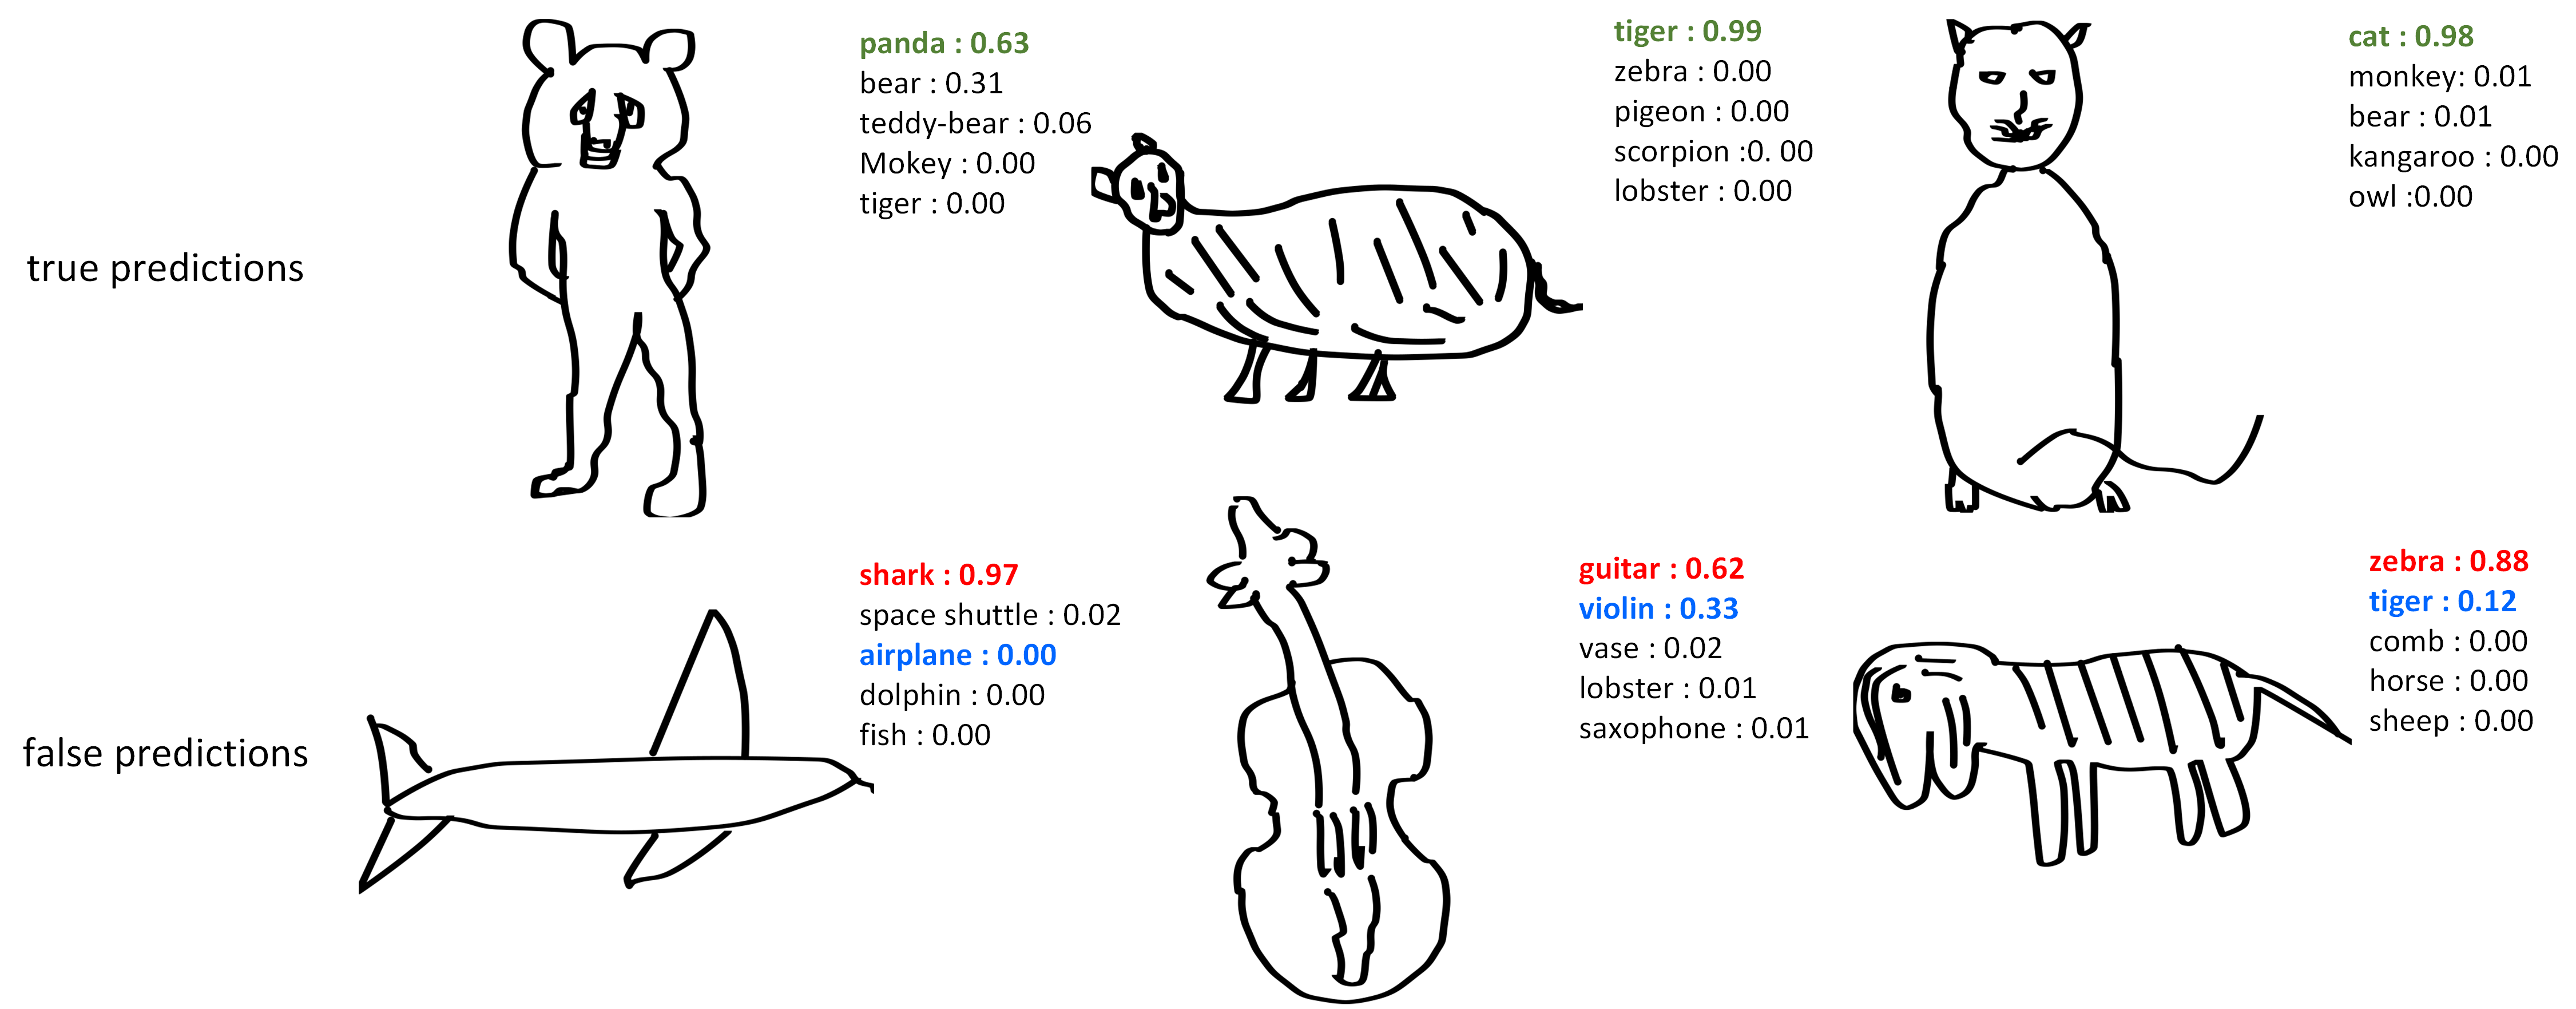
\includegraphics[width=3in]{images/res.png}
    \fcaption{Illustration of recognition successes (green) and failures (red). \cxj{revise this figure.}}
    \label{fig:resshow}
\end{figure}
